\section{Background} \label{sec:background}
In this section, we establish the essential groundwork for comprehending the intricacies of model poisoning through label flipping on FL. We begin by presenting important ideas required to understand its security landscape.

We examine the state of the art regarding adversarial attacks and defence mechanisms to get a practical perspective on security challenges. 
By exploring the landscape of model poisoning attacks, we will delve into attacker tactics that manipulate model updates, potentially compromising the integrity of federated learning

Finally, we explore the different aggregation techniques that are going to be employed on the practical side of this thesis.

%%%%%%%%%%%%%%%%%%%%%%%%%%%%%%%%%%%%%%%%%%%%%%%%%%%%%%
\subsection{Deep Neural Networks}
Deep Neural Networks (DNNs) are a specific type of ML algorithms, similar to Artificial Neural Networks, but characterized by their incorporation of multiple hidden layers situated between the input and output layers. These hidden layers allow DNNs to acquire intricate and refined data representations during training.
% Cita exemples d'ús
This inherent capability enhances their performance across diverse domains, encompassing healthcare \cite{BreastCancerComputerVision}, game playing \cite{gamePlaying}, speech recognition \cite{speechRecognition}, analysis of molecular structures and predicting chemical properties \cite{MolecularStructure}, and recommendation systems \cite{DNNRecommendation}, among many others.

% Reescrit això, faltaria alguna referencia a algún llibre o curs
Formally, a DNN applies a series of nested non-linear operations between the inputs and a collection of tunable parameters, called weights and biases. Given an input vector $x$, a weight vector $w$, and a bias vector $b$, a neuron computes $o=\sigma(\sum_i x_i w_i + b)$, where $\sigma(\cdot)$ is a non-linear function, such as the sigmoid function, the hyperbolic tangent function, or the Rectified Linear Unit (which equals 0 for negative inputs and the identity for non-negative inputs).
During training, an optimization algorithm, such as stochastic gradient descent, is used to minimize a loss function, that is, a function that scores how close are the predictions of the model with respect to the expected ones.
These optimization algorithms alternate forward and backward passes in which the loss function is computed on some training examples and the expected results, the derivative of the loss function with respect to the model parameters is computed, and the weights and biases are adjusted according to the computed gradients and a configurable learning rate. These forward and backward passes are repeated until the model converges or reaches an acceptable level of loss or predictive power. \autoref{fig:DNN_example} shows a representation of a DNN that classifies images into classes of animals.

Specialized architectures, such as convolutional neural networks, recurrent neural networks, or transformers use special layers to solve particular problems, such as image recognition, time series analysis, or natural language processing.

% The DNN first creates a map of artificial neurons and, assigns to the connections linking them initial random "weights", or numerical values. These weights interact with the inputs to produce an output that can range from 0 to 1. An algorithm intervenes to adjust these weights if the network is unable to recognise a particular pattern with sufficient accuracy. Through this procedure, the algorithm can gradually increase the influence of specific parameters while iteratively determining the most effective mathematical operations necessary to efficiently process the input data. \autoref{fig:DNN_example} shows a representation of a DNN that classifies images into classes of animals.

For instance, a DNN trained to recognise plant species will examine the supplied image and determine whether the plant in the image is a member of a particular species. The user can then evaluate the outcomes and select the probabilities that the network should present (those that are higher than a certain threshold, etc.), resulting in the suggested label.
\begin{figure}[h!]
        % \begin{figure}[H] % Alternative positioning
        \centering % sempre
        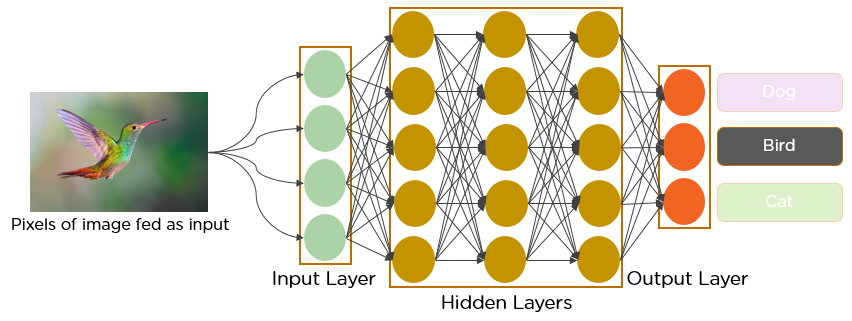
\includegraphics[scale=0.45]{DNN_example.png}
        \caption{Deep Neural Network representation. Source: \textit{Analytics Vidhya}} % sempre
        \label{fig:DNN_example}
\end{figure}


%%%%%%%%%%%%%%%%%%%%%%%%%%%%%%%%%%%%%%%%%%%%%%%%%%%%%%
\subsection{Federated Learning}
Federated Learning, first proposed by McMahan et al. in 2017 \cite{FederatedLearningPaper}, has become recognised as an innovative paradigm in the context of ML. In the age of distributed computing and data privacy concerns, FL offers an innovative approach of model training. By allowing ML models to be trained collaboratively across decentralised devices while protecting the confidentiality of specific data sources, it addresses the issue of centralised data ownership and the privacy implications it has.

The FL training procedure is an excellent representation of a distributed and privacy-protecting mechanism. Using their private data, participating devices or clients refine specific models in this scheme. The global model is used as the starting point for each client's training process and is initialised and distributed by a central server. Clients produce incremental model updates by iteratively optimising this global model through their local datasets. The central server receives these updates, compiles them, and distributes the new global model again to the clients. This method's elegance lies in its capacity to combine information from various data sources while protecting private data at the source.

Due to its collaborative and iterative structure, FL has special qualities that set it apart from conventional centralised learning paradigms. The training dynamics are made more complex by the presence of device-specific data distributions and a variety of client computational capabilities. Therefore, FL encompasses challenges that go beyond those of conventional ML, calling for the investigation of reliable communication protocols, secure aggregation techniques, and methods for dealing with potential adversarial threats.

Compared to conventional centralised ML approaches, FL offers several compelling advantages:

\begin{itemize}
        \item The training computational load is effectively distributed across the participating peers' devices, which is particularly important for large-scale ML tasks.
        \item Joint training on various data sources improves model accuracy and yields more accurate insights for both peers and the central server.
        \item  By eliminating the requirement to share local data with a central server, FL crucially protects individual privacy.
\end{itemize}

Due to the latter advantage, FL is particularly suitable for scenarios involving sensitive data, such as those in location-based services, voice assistants, healthcare,  facial recognition, and voice assistants. Additionally, FL is extremely useful in scenarios where data processing and collection are limited by privacy protection laws like the General Data Protection Regulation (GDPR \cite{GDPR}) by the European Commission or the Spanish "\textit{Ley Orgánica de Protección de Datos}" (LOPD).

%%%%%%%%%%%%%%%%%%%%%%%%%%%%%%%%%%%%%%%%%%%%%%%%%%%%%%%
\subsection{Privacy and security issues of Federated Learning}\label{sec:state_of_the_art}
Despite the numerous advantages that FL offers over centralised learning, the decentralised nature of this approach also creates vulnerabilities to security and privacy threats. In fact, the distributed architecture that empowers FL, can increase the impact of these attacks, surpassing the risks associated with more conventional centralised learning.

Numerous security and privacy issues can still affect FL. On the security front, the vulnerabilities include Byzantine attacks that aim to obstruct model convergence and, poisoning attacks, that are deliberately designed to influence convergence in the wrong direction.

%%%%%%%%%%%%%%%%%%%%%%%%%%%%%%%%%%%%%%%%%%%%%%%%%%%%%%%
\subsubsection{Privacy attacks}
While FL works to prevent direct sharing of private data, the process of exchanging local updates creates the possibility of sensitive information leakage to malicious actors.

The gradients computed on individual devices have the potential to unintentionally make adversaries aware of subtle aspects of the training data. Deep Learning models have an extraordinary capacity to retain information beyond what is strictly required for their primary task, and this tendency can unintentionally reveal unintended properties of the data they were trained on.

Peers' local updates reflect the understanding gained from their different training datasets. As a result, these updates have the unintentional potential to reveal personal information, such as class distributions, membership details, and inherent properties of the local training data. This unintentionally gives adversaries the ability to infer class labels by reconstructing training samples without having any prior knowledge of the underlying data.

%%%%%%%%%%%%%%%%%%%%%%%%%%%%%%%%%%%%%%%%%%%%%%%%%%%%%%%
\subsubsection{Poisoning attacks against Federated Learning}
FL is vulnerable to poisoning attacks, a technique designed to sabotage the learning process by introducing malicious data or model updates. These attacks within FL systems can be divided into two categories: untargeted and targeted.

Understanding the landscape of poisoning attacks against FL is crucial to safeguarding the integrity of the learning process. During FL's training phase, both targeted and untargeted poisoning attacks can be executed, influencing either the local model or the local data. The act of injecting manipulated samples into the training dataset is known as "data poisoning attack," capable of introducing distortions by feeding the model with inaccurate or biased data. In contrast, model poisoning attacks involve the manipulation of model parameters during the local model training, either directly or indirectly.

%%%%%%%%%%%%%%%%%%%%%%%%%%%%%%%%%%%%%%%%%%%%%%%%%%%%%%%
\subsubsection{Untargeted poisoning attacks}\label{sec:untargeted}
Untargeted poisoning attacks in the context of FL focus on degrading the model's overall performance rather than aiming for particular misclassifications. Without following a predetermined pattern, these attacks introduce noise or perturbations into the training process. The result is a compromised global model with decreased prediction accuracy and reliability.

Byzantine attacks are a subset of untargeted attacks that involve malicious devices deliberately sending false updates to the central server during the model aggregation phase. In order to prevent the convergence of the global model from happening, these malicious devices act dishonestly by transmitting updated model data that has been altered or corrupted. Unaware of the adversarial behaviour, the central server aggregates these updates, creating a distorted model that does not accurately reflect the underlying data.

Due to the hidden nature of the malicious actions, which can closely resemble legitimate participation, detecting Byzantine attacks can be challenging.  Standard aggregation techniques might unintentionally include these contaminated updates, which would make the global model perform poorly on unobserved data.

%%%%%%%%%%%%%%%%%%%%%%%%%%%%%%%%%%%%%%%%%%%%%%%%%%%%%%%
\subsubsection{Targeted poisoning attacks}\label{sec:targeted}
Targeted poisoning attacks have a specific goal: inducing the global model to misclassify a chosen set of samples into a target class chosen by the attacker.
The specific targeted attack that holds relevance for this thesis is the label-flipping attack.

In a label-flipping attack, attackers employ their local dataset to carry out their poisoning strategy in the following way: for each instance in the dataset that originally has the source class label, they meticulously change the label to the target one. These attackers then proceed to train their local models after manipulating their training data. The parameters used in this training process are the same as those provided by the central server. As a result, the model learns on these incorrectly labelled examples, which causes it to produce inaccurate predictions in the future when presented with images of a similar nature.

Consider a scenario for a medical diagnosis where a FL model is trained to distinguish between samples that are healthy and those that are diseased. A label-flipping attack could be carried out by an attacker by changing the labels of some healthy samples to read "diseased." The model then gains knowledge from these falsified data, misclassifying real healthy samples as diseased during inference. In real-world applications, such as incorrect diagnoses or treatment recommendations, such a scenario might have serious consequences. 

%%%%%%%%%%%%%%%%%%%%%%%%%%%%%%%%%%%%%%%%%%%%%%%%%%%%%%%
\subsubsection{Defences against poisoning attacks}\label{sec:defenses}
The way for a malicious actor to compromise the integrity of the learning process is, as seen in the previous sections \ref{sec:untargeted} and \ref{sec:targeted}, by injecting poisoned data on local model updates. The attacker must also overcome the combined influence of benign clients during the aggregation process in order ensure a successful attack. This can be done in a number of ways, including:
\begin{itemize}
        \item Applying scaling factors to boost the impact of their own updates.
        \item Colluding with other malicious clients, whether they are additional accounts linked to the same attacker or different attackers themselves.
        \item Applying a combination of the aforementioned strategies.
\end{itemize}

A useful strategy to prevent attacks of this nature would be, given that the server possesses the unique identifier (ID) of peers participating in the current training round, contrasting the model's accuracy results with those of prior rounds. In rounds of noteworthy disparities, the algorithm could store the IDs of participants from that specific round. In subsequent rounds marked by discrepancies, this stored list could be cross-referenced with the current round IDs, allowing for the removal of IDs not actively participating in the ongoing round. This strategy would eventually facilitate the detection of a single malicious peer. Notably, this identification does not require to ban the detected malicious peer, as this might lead her to create a new account to evade detection.
For scenarios involving multiple malicious peers, an iterative process would take place, persisting until the identification of additional attackers is achieved. To establish a trustable first global round for future comparisons, the server could initiate this round with the assurance of a lack of attackers at the chosen peers set.


A less 'drastic' approach to blacklisting is using reputations, rewarding good updates and penalizing bad ones, and during aggregation, weighting updates based on peers' reputations. Thus, updates from suspicious peers carry less weight than those from trustworthy ones.
The issue with this mechanism is that it assumes the central server has access to sufficient testing data for model evaluation. In a FL setting, this does not always hold true, which is why the mechanisms discussed below have been proposed.



The strategies for defending against poisoning attacks that have been suggested in the literature follow one of the following principles:
\begin{itemize}
        \item Update Aggregation: In this method, local model updates are aggregated using methods that are robust to outliers. The impact of inaccurate updates on the final global model is reduced by using aggregation techniques that are resilient to extreme values. This ensures that the effects of potentially harmful updates are minimised, allowing to produce an aggregated model that is more reliable and accurate.
        \item Evaluation Metrics: The central idea of this approach is to evaluate the quality of local updates using evaluation metrics connected to the global model. The model aggregation process may exclude or penalise a local update if it negatively impacts a certain metric, such as accuracy.
        \item Update Clustering: In a different approach, updates are split into two clusters, with the smaller cluster being marked as potentially malicious and ignored during model learning. This idea helps filter out potentially harmful updates.
        \item Peers' Behaviour: This approach makes the assumption that malicious peers behave similarly, which makes their updates more similar than those of honest peers. In order to reduce the impact of potentially harmful updates, penalization is therefore based on the similarity between updates.
        \item Differential Privacy (DP): Using the DP method, each update parameter is altered by being clipped to a maximum threshold and then introducing random noise. As a result, there is a compromise between the ability of the aggregated model to perform its main task and the mitigation of potential attacks through added noise.
\end{itemize}

The strategies implemented in the base code that is used in this thesis \cite{LFighter_code} are:
\begin{itemize} \label{sec:aggregation_methods}
        \item Federated Averaging (FedAvg) \cite{FederatedLearningPaper}: The standard aggregation method used in FL. It works by aggregating the local updates by averaging them. This method is not designed to counter poisoning attacks.
        \item Median \cite{MedianPaper}: This strategy involves collecting local model updates from participating devices and determining the median value for each parameter across these updates. After sorting the parameter values, the median strategy selects the middle value while ignoring extreme outliers. Since a single adversarial device cannot significantly impact the final aggregated model, this method makes the median aggregation resistant to malicious or inaccurate updates.
        \item Trimmed Mean (TMean) \cite{MedianPaper}: This method decreases the impact of outliers by excluding a certain percentage of extreme values. By reducing the impact of potentially malicious updates or noisy data from individual devices, this strategy improves the robustness of the aggregation process.
        \item Multi-Krum (MKrum) \cite{MKrumPaper}: The updates chosen for aggregation using this method are the most agreeable ones. The algorithm isolates potentially malicious or abnormal updates by selecting a subset of updates with the highest consensus among participating devices. The MKrum strategy improves the robustness of aggregation against adversarial behaviour and data anomalies by focusing on the level of agreement among multiple devices.
        \item FoolsGold (FGold) \cite{FoolsGoldPaper}: By taking into account the similarity of their contributions, the method adapts the learning rate of clients. The central idea of this strategy is based on the notion that when a group of sybils\footnote{A term used in computer security to describe a scenario in which a user or entity generates several different entities.} manipulates a shared model, their updates over the course of training will align towards a particular malicious objective, displaying a higher degree of similarity than expected. In FL, it serves as a robust defence mechanism against assaults planned by any number of sybils.
        \item Tolpegin \cite{TolpeginPaper}: The weights associated with the potentially targeted source class are examined by this method using Principal Component Analysis (PCA)\footnote{PCA  is a statistical technique used to reduce the dimensionality of data while preserving its essential features.}. Within those weight distributions, it selectively eliminates potential adversarial updates that deviate from the prevailing trend.
        \item FLAME \cite{FLAMEPaper}: Model clustering and weight clipping are two techniques FLAME employs to reduce the required noise infusion. This method accomplishes two goals through this method: successfully closing any potential adversarial backdoors while maintaining the aggregate model's desirable performance.
        \item LFighter \cite{ThesisNajeeb}: This method effectively filters out updates that might be harmful before model aggregation by extracting gradients corresponding to potential source and target classes from local updates, clustering them. It's noteworthy that this proposed defence is robust across various data distributions and model dimensions.
\end{itemize}




















% \subsubsection{types of fl}
% Types of FL. Federated Learning is not limited to the horizontal FL framework. Several other types of FL frameworks have been developed to handle different scenarios (Mammen, 2021):
% • Horizontal federated learning (HFL): This is used when each peer has a data set with the same feature space but different sample instances. A classic use case is the Google Keyboard app, where participating mobile phones have different training data but the same features.
% • Vertical federated learning (VFL): This is used when each peer has a data set with different features but from the same sample in- stances. For example, two organizations with data about the same group of people but with different feature sets can use Vertical FL to build a shared ML model.
% • Federatedtransferlearning(FTL):ThisissimilartotraditionalML, where we want to add a new feature to a pre-trained model. An example of this is extending Vertical FL to include more sample instances that are not present in all collaborating organizations.
% • Cross-silo federated learning: This is a type of FL where partic- ipating peers are large distributed entities (e.g., hospitals, banks, and companies) that have abundant local data and computational resources, and are available for all rounds. The training data can be in horizontal or vertical FL format.
% • Cross-device federated learning: This is another type of FL where peers are small distributed entities (e.g., smartphones, wearables, and edge devices) that have limited local data and computational resources. In this type, the number of peers is large, and they are not available for all rounds. Usually, the training data are in hori- zontal FL format.


% \subsubsection{Security attacks on Federated Learning}

% Despite these advantages, FL is vulnerable to various security and pri- vacy attacks \\
% Regarding security, FL is vulnerable to poisoning attacks 
% (Blanco- Justicia et al., 2021; Lyu et al., 2022). Since the server has no control
%  over the behavior of the participating peers, any of them may deviate from the prescribed 
%  training protocol to attack the global model by conduct- ing either untargeted poisoning 
%  attacks (Blanchard et al., 2017; Wu et al., 2020b) or targeted poisoning attacks \\

% In the former type of attacks, the attacker aims to degrade the model’s over- all 
%  performance, whereas in the latter, he aims to cause the global model to misclassify 
%  some attacker-chosen inputs into an attacker-chosen class.\\

% Furthermore, poisoning attacks can be performed in two ways: model poisoning 
%  (Blanchard et al., 2017; Wu et al., 2020b; Bagdasaryan et al., 2020) or data poisoning\\

%  In model poisoning, the attackers maliciously manipulate their local model parameters 
%  before sending them to the server. In data poisoning, they inject fabricated or falsified 
%  data samples into their training data before local model train- ing. Both attacks result 
%  in poisoned updates being uploaded to the server in order to prevent the global model from 
%  converging or to bias\\

%  As FL becomes more prevalent in real-world applications, safeguard- ing its models against poisoning and privacy attacks becomes crucial.
%  Several defenses against poisoning attacks have been proposed\\

%  Most of these defenses are effective against un- targeted poisoning attacks, but they impose a high computational cost on the server to filter out poisoned updates.\\

%  Moreover, they often become less effective or even fail against targeted poisoning attacks such as label- flipping attacks (LFs) or backdoor attacks (BAs)\\

% We can use techniques such as homomorphic encryption or secure multiparty computation
% which securely aggregate updates before sending them to the server but, 
% these techniques are computationally expensive and prevent the server from inspecting
%  individual updates to detect and filter out poisoned ones.\\

% To detect poisoning attacks, the server requires direct access to individual updates

% Therefore, simultaneously achieving security, privacy and accuracy is a tough challenge for FL.\\

\pagebreak